\documentclass{ltxdockit}
\usepackage[british]{babel}
\usepackage[strict=true,autostyle=true]{csquotes}
\usepackage{ifthen}
\usepackage{fontspec}
\usepackage{graphicx}
\usepackage{booktabs}
\setmainfont[Ligatures=TeX]{TeXGyrePagella}
\setsansfont{Arial}
\setmonofont{Courier New}

\MakeAutoQuote{«}{»}

\titlepage{%
  title={biber},
  subtitle={A backend bibliography processor for biblatex},
  url={http://biblatex-biber.sourceforge.net},
  author={François Charette, Philip Kime},
  email={firmicus@ankabut.net, Philip@kime.org.uk},
  revision={biber 0.6.4},
  date={\today}}

\hypersetup{%
  pdftitle={biber},
  pdfsubject={A backend bibliography processor for biblatex},
  pdfauthor={Philip Kime},
  pdfkeywords={biblatex, bibliography}}


% Control list spacing
\usepackage{enumitem}
\setdescription{noitemsep}
\setenumerate{noitemsep}
\setitemize{noitemsep}

\def\biberex#1{\hbox{\hspace{-4em}\texttt{\small \detokenize{#1}}}}

\begin{document}

\printtitlepage
\tableofcontents

\section{Introduction}
\label{int}

\subsection{About}

\verb+biber+ is conceptually a \verb+bibtex+ replacement for
\verb+biblatex+. It is written in Perl with the aim of providing a
customised and sophisticated data preparation backend for \verb+biblatex+.
Functionally, it offers a superset of \verb+bibtex+'s capabilities but is
tightly coupled with \verb+biblatex+ and cannot be used as a stand-alone tool
with standard \verb+.bst+ styles.

\subsection{Requirements}\label{ref:req}

\verb+biber+ is distributed in two ways. There is a Perl source
version which requires you to have a working Perl installation
(preferably version 5.12 but no less than 5.10) and the ability to
install the pre-requisite modules. Also provided are binaries for
major OSes built with the Perl \verb+PAR::Packer+ module and utilities.

Currently there are binaries available for:

\begin{itemize}
\item OSX Intel 64-bit
\item Windows
\item Linux 32-bit
\item Linux 64-bit
\end{itemize}

These should work on any fairly recent OS version. Both binaries and
Perl source are available on SourceForge\footnote{\url{http://sourceforge.net/projects/biblatex-biber/}}.

\subsection{License}

\verb+biber+ is released under the free software Artistic License 2.0\footnote{\url{http://www.opensource.org/licenses/artistic-license-2.0.php}}

\subsection{History}

\verb+bibtex+ has been the default (only \ldots) integrated choice for
bibliography processing in TeX for a long time. It has well known
limitations which stem from its data format, data model and lack of Unicode
support\footnote{In fact, there is now a Unicode version}. The
\verb+.bst+ language for writing bibliography styles is painful to learn
and use. It is not a general programming language and this makes it really
very hard to do sophisticated automated processing of bibliographies.

\verb+biblatex+ was a major advance for LaTeX users as it moved much
of the bibliography processing into LaTeX macros. However,
\verb+biblatex+ still used \verb+bibtex+ as a sorting engine for the
bibliography and also to generate various labels for
entries. \verb+bibtex+'s capabilities even for this reduced set of
tasks was still quite restricted due to the lack of Unicode support and
the more and more complex programming issues involved in label
preparation and file encoding.

\verb+biber+ was designed specifically for \verb+biblatex+ in order to
provide a powerful backend engine which could deal with any required
tasks to do with \verb+.bbl+ preparation. It can

\begin{itemize}
\item Deal with the full range of UTF-8
\item Sort in a completely customisable manner, using when available,
  CLDR collation tailorings
\item Automatically encode the \verb+.bbl+ into any supported encoding
  format\footnote{«Supported» here means encodings supported by the
    Perl \texttt{Encode} module}
\item Process all bibliography sections in one pass of the tool
\item Handle UTF-8 citekeys and filenames (given a suitable fully
  UTF-8 compliant TeX engine)
\item Handle very complex auto-expansion and contraction of names and
  namelists.
\item Lots of other things
\end{itemize}

\subsection{Acknowledgements}

François Charette originally wrote \verb+biber+. Philip Kime joined in
the development in 2009.

\section{Use}

Firstly, running \verb+biber --help+ will display all options and a brief
description of each. This is the most useful brief source of usage
information. \verb+biber+ returns an exit code of 0 on success or 1 if
there was an error.

Most \verb+biber+ options can be specified in long or short format. When
mentioning options below, they are referred to as
«\verb+long form|short form+» when an option has both a long and short
form. As usual with such options, when the option requires an argument, the
long form is followed by an equals sign «\verb+=+» and then the argument,
the short form is followed by a space and then the argument. For example,
the \verb+--bibdata|-d+ option can be given in two ways:

\begin{verbatim}
biber --bibdata=somefile.bib
biber -d somefile.bib
\end{verbatim}

With the \verb+backend=biber+ option, \verb+biblatex+ switches its backend
interface and passes all options and information relevant to \verb+biber+'s
operation in a control file with extension \verb+.bcf+\footnote{BibLaTeX Control
  File}. This is conceptually equivalent to the \verb+.aux+ file which
LaTeX uses to pass information to \verb+bibtex+. The \verb+.bcf+ file is
XML and contains many options and settings which configure how \verb+biber+
is to process the bibliography and generate the \verb+.bbl+ file.

The usual way to call \verb+biber+ is simply with the \verb+.bcf+ file
as the only argument. The «\verb+.bcf+» extension of the control file
is not optional. \verb+biblatex+ always outputs a control file with
the \verb+.bcf+ extension. Specifying the «\verb+.bcf+» extension to
\verb+biber+ \emph{is} optional. Assuming a control file called
\verb+test.bcf+, the following two commands are equivalent:

\begin{verbatim}
biber test.bcf
biber test
\end{verbatim}

\subsection{Options and config file}
\verb+biber+ sets its options using the following resource 
chain which is given in decreasing precedence order:\\[2ex]

\noindent command line options $\rightarrow$\\
\hspace*{1em}\verb+.bcf+ file$\rightarrow$\\
\hspace*{2em}\verb+biber.conf+ file $\rightarrow$\\
\hspace*{3em}\verb+biber+ hard-coded defaults\\[2ex]

\noindent Users do not need to care directly about the contents or format of the
\verb+.bcf+ file as this is generated from the options which they specify
for \verb+biblatex+. To override the \verb+.bcf+ options or to provide
option settings when no \verb+.bcf+ file is used (see for example the
\verb+--allentries|-a+ and \verb+--bibdata|-d+ options), users
may use either a configuration file or the command line to set options.

The configuration file is by default called \verb+biber.conf+ but this can
be changed using the \verb+--configfile|-g+ option. Unless
\verb+--configfile|-g+ is used, the config file is
looked for in the following places, in decreasing order of preference:\\[2ex]

\noindent \verb+biber.conf+ in the current directory $\rightarrow$\\
\hspace*{1em}\verb+$HOME/.biber.conf+ $\rightarrow$\\
\hspace*{2em}\verb+$XDG_CONFIG_HOME/biber/biber.conf+ $\rightarrow$\\
\hspace*{3em}\verb+$HOME/Library/biber/biber.conf+ (Mac OSX only)\\
\hspace*{3em}\verb+$APPDATA/biber.conf+ (Windows only) $\rightarrow$\\
\hspace*{4em}the output of \verb+kpsewhich biber.conf+ (if available on the
system)\\[2ex]

\noindent The config file format is a very flexible one which allows users to specify
options in most common formats, even mixed in the same file. It's easier to
see an example. Here is a config file which displays the \verb+biber+
hard-coded defaults:

\begin{verbatim}
allentries          0
bibdata             undef
bibdatatype         bibtex
bblencoding         UTF-8
bibencoding         UTF-8
collate             1
<collate_options>
    level           3
</collate_options>
debug               0
fastsort            0
mincrossrefs        2
nolog               0
nosortdiacritics    [\x{2bf}\x{2018}]
nosortprefix        \p{L}{2}\p{Pd}
onlylog             0
quiet               0
sortcase            true
sortlocale          en_US.utf8
sortupper           true
trace               0
validate_control    0
validate_structure  0
wraplines           0
\end{verbatim}

\noindent You can see here that options with multiple key/value pairs of
their own like\linebreak[4] \verb+--collate_options|-c+ can be specified in
Apache config format. Please see the documentation
for the \verb+Config::General+ Perl
module\footnote{\url{http://search.cpan.org/search?query=Config::General&mode=all}}
if you really need details. In practise, if you use a config file at all
for \verb+biber+, it will contain very little as you will usually set all
options by setting options in \verb+biblatex+ which will pass them to
\verb+biber+ via the \verb+.bcf+ file.

The \verb+--collate_options|-c+ option takes a number of key/value pairs as
value. See section \ref{coll} for details. The value of the \verb+nosort*+
options can only be set in the config file and not on the command line.
This is because the values are Perl regular expressions and would need
special quoting to set on the command line. This can get a bit tricky on
some OSes (like Windows) so it's safer to set them in the config file. In
any case, it's unlikely you would want to set them for particular
\verb+biber+ runs; they would more likely be set as your personal default
and thus they would naturally be set in the config file anway. They specify
stand-alone diacritic marks and name prefices to strip before sorting takes
place and are designed to deal with cases like

\begin{verbatim}
  author	   = {{al-Hasan}, ʿAlī},
\end{verbatim}

\noindent where the prefix «al-» and the diacritic «ʿ» should not be
considered when sorting.

\subsection{Input/Output File Locations}

\subsubsection{Control file}\label{loc:cf}

The control file is normally passed as the only argument to biber
(unless using \verb+--allentries|-a+ and \verb+--bibdata|-d+). It is
searched for using the following locations, in decreasing order of
priority:\\[2ex]

\noindent Absolute filename $\rightarrow$\\
\hspace*{1em}In the \verb+--output_directory+, if specified$\rightarrow$\\
\hspace*{2em}Relative to current directory$\rightarrow$\\
\hspace*{3em}Using \verb+kpsewhich+, if available

\subsubsection{Database files}

Bibliography database files are searched for using the same rule as for
control files (see section \ref{loc:cf} above). Unless using the
\verb+--bibdata|-d+ option, users usually do not specify explicitly the
bibliography database files; they are normally passed in the \verb+.bcf+
control file, taken from the \verb+biblatex + \verb+\bibliography{}+
command arguments.

\subsection{Logfile}

By default, the logfile for biber will be named \verb+\jobname.blg+,
so, if you run

\begin{verbatim}
  biber <options> test.bcf
\end{verbatim}

\noindent then the logfile will be called «\verb+test.blg+». Like the
\verb+.bbl+ output file, it will be created in the
\verb+--output_directory|-c+, if this option is defined. If there is
no \verb+.bcf+ file on the command line (for example, when using the
\verb+--allentries|-a+ and \verb+--bibdata|-d+ options), then the
logfile name will default to «\verb+biber.blg+». You can
override the logfile name by using the \verb+--logfile+ option:

\begin{verbatim}
  biber --logfile=lfname test.bcf
\end{verbatim}

\noindent results in a logfile called «\verb+lfname.blg+».

\subsection{Collation and Localisation}\label{coll}

\verb+biber+ takes care of collating the bibliography for
\verb+biblatex+. It writes entries to the \verb+.bbl+ file sorted by a
completely customisable set of rules which are passed in the
\verb+.bcf+ file by \verb+biblatex+. \verb+biber+ has two ways of performing
collation:\\[2ex]

\biberex{--collate|-C}
  \noindent The default. This option makes \verb+biber+ use the
  \verb+Unicode::Collate+ module for collation which implements the full UCA (Unicode
  Collation Algorithm). It also has CLDR (Common Locale Data
  Repository) tailoring to deal with cases which are not covered by the
  UCA. It is a little slower than \verb+--fastsort|-f+ but the
  advantages are such that it's rarely worth using \verb+--fastsort|-f+\\[1ex]

\biberex{--fastsort|-f}
  \noindent Biber will sort using
  the OS locale collation tables. The drawback for this method is that special
  collation tailoring for various languages are not implemented in the
  collation tables for many OSes. For example, few OSes correctly sort 'å'
  before 'ä' in the Swedish (\verb+sv_SE+) locale. If you are using a
  common latin alphabet, then this is probably not a problem for you.\\[2ex]

\noindent The locale used for collation is determined by the following resource
chain which is given in decreasing precedence order:\\[2ex]

\noindent\verb+--collate_options|-c+ (e.g. \verb+-c 'locale => "de_DE"'+) $\rightarrow$\\
\hspace*{1em}\verb+--sortlocale|-l+ $\rightarrow$\\
\hspace*{2em}\verb+LC_COLLATE+ environment variable $\rightarrow$\\
\hspace*{3em}\verb+LANG+ environment variable $\rightarrow$\\
\hspace*{4em}\verb+LC_ALL+ environment variable\\[2ex]

\noindent With the default \verb+--collate|-C+ option, the locale will
be used to look for a collation tailoring for that locale. It will generate an
informational warning if it finds none. This is not a problem as the vast
majority of collation cases are covered by the standard UCA and many
locales neither have nor need any special collation tailoring.

With the \verb+--fastsort|-f+ option, the locale will be
used to locate an OS locale definition to use for the collation. This
may or may not be correctly tailored, depending on the locale and the OS.\\[1ex]

\noindent Collation is by default case sensitive. You can turn this
off using the \verb+biber+ option \verb+--sortcase=false+ or from
\verb+biblatex+ using its option \verb+sortcase=false+.\\[1ex]

\noindent\verb+--collate|-C+ by default collates uppercase before
lower. You can reverse this using the \verb+biber+ option \verb+--sortupper=false+
or from \verb+biblatex+ by using its option \verb+sortupper=false+. Be
aware though that some locales rightly enforce a particular setting for
this (for example, Danish). You will be able to override it but
\verb+biber+ will warn you if you do.\\[1ex]

There are in fact many options to \verb+Unicode::Collate+
which can tailor the collation in various ways in
addition to the locale tailoring which is automatically performed.
Users should see the the documentation to the module for the various
options, most of which the vast majority of users will never
need\footnote{For details on the various options, see
  \url{http://search.cpan.org/search?query=Unicode\%3A\%3ACollate&mode=all}}.
Options are passed using the \verb+--collate_options|-c+ option as a
single quoted string, each option separated by comma, each key and
value separated by «\verb+=>+». See examples.

\subsubsection{Examples}

\biberex{biber}

\noindent Call biber using all settings from the \verb+.bcf+ generated from the
LaTeX run. Case sensitive UCA sorting is performed taking the locale
for tailoring from the environment if no \verb+sortlocale+ is defined in
the \verb+.bcf+

\biberex{biber --sortlocale=de_DE}

\noindent Override any locale setting in the \verb+.bcf+ or
the environment.

\biberex{biber --fastsort}

\noindent Use slightly quicker internal sorting routine. This uses the OS locale
files which may or may not be accurate.

\biberex{biber --sortcase=false}

\noindent Case insensitive sorting.

\biberex{biber --sortupper=false --collate_options="backwards => 2"}

\noindent Collate lowercase before upper and collate French accents in
reverse order at UCA level 2.

\subsection{Encoding of files}

\verb+biber+ takes care of reencoding the \verb+.bib+ data as
necessary. In normal use, \verb+biblatex+ passes its
\verb+bibencoding+ option value to \verb+biber+ via the \verb+.bcf+
file. It also passes an option \verb+bblencoding+ the value of which
is derived from the \verb+inputenc+ package setting (if the user is
using this package), otherwise «utf8» (for XeTeX or LuaTeX) or
«ascii» (any other TeX engine).

\noindent \verb+biber+ performs the following tasks:

\begin{enumerate}
\item Decodes the \verb+.bib+ into UTF-8 if it is not UTF-8 already
\item Decodes LaTeX character macros into UTF-8
\item Encodes the output so that the \verb+.bbl+ is in
  the encoding that \verb+bblencoding+ specifies
\item Warns if it is asked to output to the \verb+.bbl+ any UTF-8
  decoded LaTeX character macros which are not in the
  \verb+bblencoding+ encoding. Replaces with a diacritic-stripped substitute
\end{enumerate}

\noindent As you can see from item 2 above, by default, \verb+biber+
converts LaTeX character macros into UTF-8 internally. This is very
useful as it means that things are sorted correctly but has two
potential (but rare) problems which you should be aware of:

\begin{itemize}
\item If you are using PDFLaTeX and \verb+\usepackage[utf8]{inputenc}+, it
  is possible that the UTF-8 characters resulting from \verb+biber+'s
  internal LaTeX character macro decoding break \verb+inputenc+. This
  is because \verb+inputenc+ does not implement all of UTF-8, only a
  commonly used subset. 

  An example--if you had \verb+\DJ+ in your \verb+.bib+,
  \verb+biber+ decodes this correctly to «Đ» and this breaks \verb+inputenc+
  because it doesn't understand that UTF-8 character. The solution
  here is to switch to a TeX engine with full UTF-8 support like XeTeX or
  LuaTeX as these don't use or need \verb+inputenc+.
\item If your \verb+bblencoding+ is not UTF-8, and you are using some
  UTF-8 equivalent LaTeX character macros in your \verb+.bib+, then
  some \verb+.bbl+ fields (currently only \verb+\sortinit{}+) might
  end up with invalid characters in them, according to the \verb+.bbl+
  encoding. This is because some fields must be generated from the
  final sorting data which is only available after the LaTeX character
  macro decoding step.

  For example, suppose you were using PDFLaTeX with\\
  \verb+\usepackage[latin1]{inputenc}+ and the following
  \verb+.bib entry+

  \begin{verbatim}
    @BOOK{citekey1,
      AUTHOR = {{\v S}imple, Simon},
    }
  \end{verbatim}

  \noindent With normal LaTeX character macro decoding, the
  \verb+{\v S}+ is decoded into «Š» and so with name-first sorting,
  \verb+\sortinit{}+ would be «Š». This is an invalid character in
  latin1 encoding and so the \verb+.bbl+ would be broken. In such
  cases when \verb+\sortinit{}+ is a char not valid in the
  \verb+bblencoding+, \verb+biber+ strips off any diacritics which in
  this case results in «S». This is not ideal as this is not the
  initial character of the string used for sorting any more but it's a
  decent replacement in such cases. The solution is really
  to use UTF-8 \verb+bblencoding+ wherever possible. In extreme cases like
  the one above, this might also mean switching TeX engines to one that
  supports full UTF-8.
\end{itemize}

\noindent Normally, you do not need to set the encoding options on the
\verb+biber+ command line as they are passed in the \verb+.bcf+ via
the information in your \verb+biblatex+ environment. However, you can
override the \verb+.bcf+ settings with the command line or config
file. The resource chain for encoding settings is, in decreasing order
of preference:\\[2ex]

\noindent\verb+--bibencoding|-e+ and \verb+--bblencoding|-E+ $\rightarrow$\\
\hspace*{1em}\verb+biber+ config file $\rightarrow$\\
\hspace*{2em}\verb+.bcf+ control file

\subsubsection{Examples}

\biberex{biber}

\noindent Read \verb+bibencoding+ and \verb+bblencoding+ from the
config file or \verb+.bcf+.

\biberex{biber --bblencoding=latin2}

\noindent Encode the \verb+.bbl+ as latin2, overriding the
\verb+.bcf+.

\biberex{biber -u}

\noindent Shortcut alias for \verb+biber --bibencoding=UTF-8+

\biberex{biber -U}

\noindent Shortcut alias for \verb+biber --bblencoding=UTF-8+

\subsection{Limitations}

Currently, users are restricted to the bibliography entry types hard-coded
into \verb+biblatex+. This is mitigated a little by the custom fields
listed in section 2.2.4 of the \verb+bibatex+ manual but these are not
portable or semantically obvious in their meaning. It is planned to have a
customisable interface in \verb+biblatex+ which will allow users to define
entry types an fields and have these passed through to \verb+biber+ which
will validate the structure of the bibliography against these definitions.
This would allow a fully customisable data model interface. Currently this
is impossible due to a reliance on the \verb+.bib+ format which is quite
restricted in scope and extensibility. It is likely that \verb+biblatex+
and \verb+biber+ will move to a modular data layer with an XML format as
the default. \verb+.bib+ support will be maintained as a legacy format.

Currently it is not possible to automatically expand name lists to their
minimally unique truncation which is required by some styles (APA for
example). This is quite a hard problem, a solution to which is implemented
in an experimental \verb+biber+ branch but which also needs \verb+biblatex+
support, envisaged for version 2.x. It requires an enhanced \verb+.bbl+
format, amongst other things.

\subsection{Editor Integration}

Here is some information on how to integrate \verb+biber+ into some of the
more common editors

\subsubsection{Emacs}

Emacs has the very powerful AUcTeX mode for editing TeX and running
compilations. BibTeX is already integrated into AUCTeX and it is quite
simple to add support for\verb+biber+. Use the Emacs Customise interface to
modify the \verb+TeX-command-list+ variable and add a \verb+Biber+ command.

\begin{verbatim}
M-x customise-variable
TeX-command-list
\end{verbatim}

\noindent and then \verb+Ins+ somewhere a new command that looks like
Figure \ref{fig:biber-auctex}.

\begin{figure}[!htbp]
  \centering
  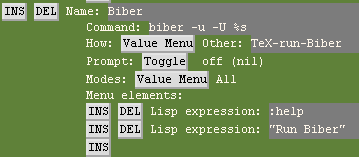
\includegraphics[width=4in,keepaspectratio=true]{biber-auctex.png}
  \caption{Screenshot of AUCTeX command setup for Biber}
  \label{fig:biber-auctex}
\end{figure}

\noindent Alternatively, you can add it directly in lisp to your \verb+.emacs+ like
this:

\begin{verbatim}
(add-to-list 'TeX-command-list
  (quote
    ("Biber" "biber %s" TeX-run-Biber nil t :help "Run Biber")))
\end{verbatim}

\noindent However you add the command to \verb+TeX-command-list+, customise the
actual \verb+Biber+ command parameters as you want them, using ``\verb+%s+" as
the LaTeX file name place holder. Then define the following two functions
in your \verb+.emacs+.

\begin{verbatim}
; Biber under AUCTeX
(defun TeX-run-Biber (name command file)
  "Create a process for NAME using COMMAND to format FILE with Biber." 
 (let ((process (TeX-run-command name command file)))
    (setq TeX-sentinel-function 'TeX-Biber-sentinel)
    (if TeX-process-asynchronous
	process
      (TeX-synchronous-sentinel name file process))))

(defun TeX-Biber-sentinel (process name)
  "Cleanup TeX output buffer after running Biber."
  (goto-char (point-max))
  (cond
   ;; Check whether Biber reports any warnings or errors.
   ((re-search-backward (concat
			 "^(There \\(?:was\\|were\\) \\([0-9]+\\) "
			 "\\(warnings?\\|error messages?\\))") nil t)
    ;; Tell the user their number so that she sees whether the
    ;; situation is getting better or worse.
    (message (concat "Biber finished with %s %s. "
		     "Type `%s' to display output.")
	     (match-string 1) (match-string 2)
	     (substitute-command-keys
	      "\\<TeX-mode-map>\\[TeX-recenter-output-buffer]")))
   (t
    (message (concat "Biber finished successfully. "
		     "Run LaTeX again to get citations right."))))
  (setq TeX-command-next TeX-command-default))
\end{verbatim}

\noindent You'll then see a \verb+Biber+ option in your AUCTeX command menu or
you can just \verb+C-c C-c+ and type \verb+Biber+.

\subsubsection{TeXworks}

It's very easy to add \verb+biber+ support to TeXworks. In the Preferences,
select the Typesetting tab and then add a new Processing Tool as in Figure
\ref{fig:biber-texworks}.

\begin{figure}[!htbp]
  \centering
  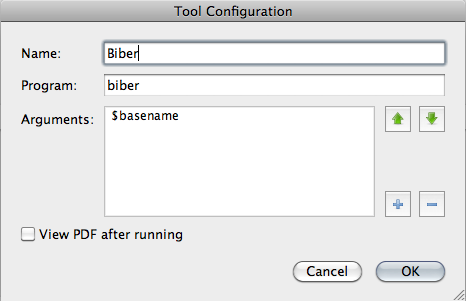
\includegraphics[width=4in,keepaspectratio=true]{biber-texworks.png}
  \caption{Screenshot of TeXworks processing tool setup for Biber}
  \label{fig:biber-texworks}
\end{figure}

\subsection{Cross-references}

\verb+biblatex+ supports the \verb+CROSSREF+ field in bibliography
databases and because \verb+biber+ performs the actual processing of such
fields, it can do this in a customisable way. Currently, the customisable
interface via user \verb+biblatex+ macros and the \verb+.bcf+ file is not
yet implemented but the internal code in \verb+biber+ is ready for this.
The purpose of this section is to describe the current hard-coded
\verb+biber+ defaults. By default, the cross-reference target (child) will
inherit all of the source (parent) fields if they are not already defined
in the target. Table \ref{tab:ct} shows the current custom
mappings which apply. These custom cross-reference mappings
will overwrite the target fields, if they exist. In future, the fully
customisable interface will allow:

\begin{itemize}
\item Choice of overwriting target fields with source fields
\item Choice of whether or not to, by default, inherit all fields from the source
\item Mapping of any source field to any target field
\item Mapping of field(s) in any source to specific targets
\item Mapping of field(s) in specific sources to any targets
\item Many-to-one and one-to-many field mappings
\item Skipping inheritance of specific source fields
\end{itemize}

\noindent The custom cross-reference mappings will make it possible to
overcome the problems with the traditional \verb+bibtex+ handling of
cross-references which are mentioned in section 2.4.1 of the
\verb+biblatex+ manual. As mentioned above, only the hard-coded mappings in
Table \ref{tab:ct} are currently implemented.

\begin{table}
\begin{center}
\small
\begin{tabular}{lllll}
\toprule
Source & Target & Source field & $\rightarrow$ & Target field\\
\midrule
\texttt{PROCEEDINGS} & \texttt{INPROCEEDINGS} & \texttt{TITLE} & $\rightarrow$ & \texttt{BOOKTITLE}\\
& & \texttt{SUBTITLE} & $\rightarrow$ & \texttt{BOOKSUBTITLE}\\
& & \texttt{TITLEADDON} & $\rightarrow$ & \texttt{BOOKTITLEADDON}\\
\cmidrule{3-5}
\texttt{COLLECTION} & \texttt{INCOLLECTION} & \texttt{TITLE} & $\rightarrow$ & \texttt{BOOKTITLE}\\
& & \texttt{SUBTITLE} & $\rightarrow$ & \texttt{BOOKSUBTITLE}\\
& & \texttt{TITLEADDON} & $\rightarrow$ & \texttt{BOOKTITLEADDON}\\
\cmidrule{3-5}
\texttt{BOOK} & \texttt{INBOOK} & \texttt{TITLE} & $\rightarrow$ & \texttt{BOOKTITLE}\\
& & \texttt{SUBTITLE} & $\rightarrow$ & \texttt{BOOKSUBTITLE}\\
& & \texttt{TITLEADDON} & $\rightarrow$ & \texttt{BOOKTITLEADDON}\\
& & \texttt{AUTHOR} & $\rightarrow$ & \texttt{BOOKAUTHOR}\\
\bottomrule
\end{tabular}
\end{center}
\caption{Custom cross-reference mappings}
\label{tab:ct}
\end{table}

\section{Binaries}

The binary distributions of biber are made using the Perl \verb+PAR::Packer+
module. They can be used as a normal binary but have some behaviour which
is worth noting:

\begin{itemize}
\item Don't be worried by the size of the binaries. \verb+PAR::Packer+ essentially
  constructs a self-extracting archive which unpacks the needed files first
  and so the binaries look larger than what actually runs in memory.
\item On the first run of a new version (that is, with a specific hash),
  they actually unpack themselves to a temporary location which varies by
  operating system. This unpacking can take a little while and only happens on
  the first run of a new version.
\end{itemize}

\subsection{Binary Caches}

\verb+PAR::Packer+ works by unpacking the required files to a cache
location. It only does this on the first run of a binary 
by computing a hash of the binary and comparing it with
the cache directory name which contains the hash. So, if you run
several versions of a binary, you will end up with several cached
trees which are never used. This is particularly true if you are regularly
testing new versions of the \verb+biber+ binary. It is a good idea to
delete the caches for older binaries as they are not needed and can take up
a fair bit of space. The caches are located in a temporary location which
varies from OS to OS. The cache name is:\\[1ex]

\noindent\verb+par-<username>/cache-<hash>+ (Linux/Unix/OSX)\\
\verb+par-<username>\cache-<hash>+ (Windows)\\[1ex]

\noindent The temp location is not always obvious but these are sensible
places to look (where \verb+*+ can vary depending on user:

\begin{itemize}
\item \verb+/var/folders/*/*/-Tmp-/+ (OSX, local GUI login shell)
\item \verb+/var/tmp/+ (OSX, remote ssh login shell)
\item \verb+/tmp/+ (Linux)
\item \verb+C:\Documents and Settings\<username>\Local Settings\Temp+ (Windows)
\item \verb+C:\Windows\Temp+ (Windows)
\end{itemize}

\noindent To clean up, you can just remove the whole \verb+par-<username>+
directory/folder and then run the current binary again.

\subsection{Binary Architectures}

Binaries are available for the following architectures:

\begin{itemize}
\item \verb+linux_x86_32+ --- Linux x86 32-bit (built on Ubuntu 9.04)
\item \verb+linux_x86_64+ --- Linux x86 64-bit (built on Ubuntu 9.04)
\item \verb+MSWin+ --- Windows. Should work on 32 or 64 bit (built on XP)
\item \verb+darwin_x86_64+ --- OSX Intel 64-bit (built on OSX 10.6)
\end{itemize}

\subsection{Installing}

These instructions only apply to manually downloaded binaries. If
\verb+biber+ came with your TeX distribution just use it as normal.

Download the binary appropriate to you
OS/arch\footnote{\url{https://sourceforge.net/projects/biblatex-biber}}. Below
I assume it's on your desktop.

You have to move the binary to somewhere in you command-line or TeX utility
path so that it can be found. If you know how to do this, just ignore the
rest of this section which contains some instructions for users who are
not sure about this.

\subsubsection{OSX}

If you are using the TexLive MacTeX distribution:

\begin{verbatim}
sudo mv ~/Desktop/biber /usr/texbin/
sudo chmod +x /usr/texbin/biber
\end{verbatim}

\noindent If you are using the macports TexLive distribution:

\begin{verbatim}
sudo mv ~/Desktop/biber /opt/local/bin/
sudo chmod +x /opt/local/bin/biber
\end{verbatim}

\noindent The «\verb+sudo+» commands will prompt you for your password.

\subsubsection{Windows}

The easiest way is to just move the executable into your \verb+C:\Windows+ directory since
that is always in your path. A more elegant is to put it somewhere in
your TeX distribution that is already in your path. For example if you
are using MiKTeX:

\begin{verbatim}
C:\Program Files\MiKTeX 2.8\miktex\bin\
\end{verbatim}

\subsubsection{Unix/Linux}

\begin{verbatim}
sudo mv ~/Desktop/biber /usr/local/bin/biber
sudo chmod +x /usr/local/bin/biber
\end{verbatim}

\noindent Make sure \verb+/usr/local/bin+ is in your PATH. Search Google for «set PATH
linux» if unsure about this. There are many pages about this, for example:
\url{http://www.cyberciti.biz/faq/unix-linux-adding-path/}


\subsection{Building}

Instructions for those who want/need to build an executable from the
Perl version. For this, you will need to have a recent Perl,
preferably 5.12 at least with the following modules:

\begin{itemize}
\item \verb+PAR+
\item \verb+PAR::Packer+
\item All \verb+biber+ pre-requisites
\end{itemize}

\noindent You should have the latest CPAN versions of all required modules
as \verb+biber+ is very specific in some cases about module versions and
depends on recent fixes in many cases. You can see if you have the
\verb+biber+ Perl dependencies by the usual

\begin{verbatim}
perl ./Build.PL
\end{verbatim}

\noindent invocation in the biber Perl distribution tree
directory. Normally, the build procedure for the binaries is as
follows\footnote{On UNIXequse systems, you may need to specify a full
  path to the scripts e.g. \texttt{./Build}}:

\begin{itemize}
\item Get the biber source tree from SF and put it on the architecture
  you are building for
\item cd to the root of the source tree
\item \verb+perl Build.PL+ (this will check your module
  dependencies)
\item \verb+Build test+
\item \verb+Build install+ (may need to run this as sudo on
  UNIXesque systems)
\item \verb+cd dist/<arch>+
\item \verb+build.sh+ (\verb+build.bat+ on Windows)
\end{itemize}

\noindent This leaves a binary called «\verb+biber-<arch>+» (also with
a «\verb+.exe+» extension on Windows) in your current directory.
The tricky part is constructing the information for the build
script. There are two things that need to be configured, both of
which are required by the \verb+PAR::Packer+ module:

\begin{enumerate}
\item A list of modules/libraries to include in the binary which are not
  automatically detected by the \verb+PAR::Packer+ dependency
  scanner
\item A list of extra files to include in the binary which are not
  automatically detected by the \verb+PAR::Packer+ dependency
  scanner
\end{enumerate}

\noindent To build \verb+biber+ for a new architecture you need to
define these two things as part of constructing new build scripts:

\begin{itemize}
\item Make a new subfolder in the \verb+dist+ directory named after the
  architecture you are building for. This name is arbitrary but should
  be fairly obvious like «\verb+solaris-sparc-64+», for example.
\item Copy the \verb+biber.files+ file from an existing build
  architecture into this directory.
\item For all of the files with absolute pathnames in there (that is,
  ones we are not pulling from the \verb+biber+ tree itself), locate these
  files in your Perl installation tree and put the correct path in the
  file.
\item Copy the build script from a vaguely similar architecture
  (i.e. Windows/non-Windows \ldots) to your new architecture
  directory. 
\item Change the \verb+--link+ options to point to where the required
  libraries reside on your system.
\item Change the \verb+--output+ option to name the resulting binary
  for your architecture.
\item Run the build script
\end{itemize}

\noindent The \verb+--link+ options can be a little tricky
sometimes. It is usually best to build without them once and then run
\verb+ldd+ (or Windows equivalent) on the binary to see which
version/location of a library you should link to. You can also try
just running the binary and it should complain about missing libraries
and where it expected to find them. Put this path into the
\verb+--link+ option. The \verb+--module+ options are the same for all
architectures and do not need to be modified.
On architectures which have or can have case-insensitive file systems,
you should use the build script from either Windows or OSX as a reference
as these include a step to copy the main \verb+biber+ script to a new name
before packing the binary. This is required as otherwise a spurious
error is reported to the user on first run of the binary due to a name
collision when it unpacks itself.

\end{document}
